% Created 2016-01-02 Sat 16:16
\documentclass[11pt]{article}
\usepackage[utf8]{inputenc}
\usepackage[T1]{fontenc}
\usepackage{fixltx2e}
\usepackage{graphicx}
\usepackage{longtable}
\usepackage{float}
\usepackage{wrapfig}
\usepackage{rotating}
\usepackage[normalem]{ulem}
\usepackage{amsmath}
\usepackage{textcomp}
\usepackage{marvosym}
\usepackage{wasysym}
\usepackage{amssymb}
\usepackage{capt-of}
\usepackage[hidelinks]{hyperref}
\tolerance=1000
\usepackage[utf8]{inputenc}
\usepackage{commath}
\usepackage{pgf}
\usepackage{tikz}
\usetikzlibrary{shapes,backgrounds}
\usepackage{marginnote}
\usepackage{listings}
\usepackage{enumerate}
\usepackage{algpseudocode}
\usepackage{algorithm}
\usepackage{mathtools}
\usetikzlibrary{arrows,automata}
\setlength{\parskip}{16pt plus 2pt minus 2pt}
\renewcommand{\arraystretch}{1.6}
\DeclareMathOperator{\Neg}{Neg}
\author{Oleg Sivokon}
\date{\textit{<2016-01-01 Fri>}}
\title{Assignment 15, Authomata Theory}
\hypersetup{
 pdfauthor={Oleg Sivokon},
 pdftitle={Assignment 15, Authomata Theory},
 pdfkeywords={Automata Theory, Formal Languages, Assignment},
 pdfsubject={Fifth assignment in the course 20440 Automata and Formal Languages},
 pdfcreator={Emacs 25.0.50.1 (Org mode 8.3beta)}, 
 pdflang={English}}
\begin{document}

\maketitle
\tableofcontents

\definecolor{codebg}{rgb}{0.96,0.99,0.8}
\definecolor{codestr}{rgb}{0.46,0.09,0.2}
\lstset{%
  backgroundcolor=\color{codebg},
  basicstyle=\ttfamily\scriptsize,
  breakatwhitespace=false,
  breaklines=false,
  captionpos=b,
  framexleftmargin=10pt,
  xleftmargin=10pt,
  framerule=0pt,
  frame=tb,
  keepspaces=true,
  keywordstyle=\color{blue},
  showspaces=false,
  showstringspaces=false,
  showtabs=false,
  stringstyle=\color{codestr},
  tabsize=2
}
\lstnewenvironment{maxima}{%
  \lstset{%
    backgroundcolor=\color{codebg},
    escapeinside={(*@}{@*)},
    aboveskip=20pt,
    captionpos=b,
    label=,
    caption=,
    showstringspaces=false,
    frame=single,
    framerule=0pt,
    basicstyle=\ttfamily\scriptsize,
    columns=fixed}}{}
}
\makeatletter
\newcommand{\verbatimfont}[1]{\renewcommand{\verbatim@font}{\ttfamily#1}}
\makeatother
\verbatimfont{\small}%
\clearpage

\section{Problems}
\label{sec:orgheadline13}

\subsection{Problem 1}
\label{sec:orgheadline3}
\begin{enumerate}
\item Show right-linear grammar equivalent to the automaton given below:

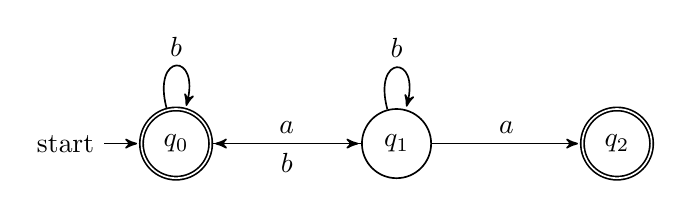
\begin{tikzpicture}[->,>=stealth',shorten >=1pt,auto,node distance=2.8cm,
                    semithick]

  \node[accepting,initial,state]   (A)              {$q_0$};
  \node[state]                     (B) [right of=A] {$q_1$};
  \node[accepting,state]           (C) [right of=B] {$q_2$};

  \path (A) edge [loop above] node {$b$} (A)
            edge              node {$a$} (B)
        (B) edge [loop above] node {$b$} (B)
            edge              node {$a$} (C)
            edge              node {$b$} (A);
\end{tikzpicture}

\item Build a finite automaton for the language given by the grammar rules:
\begin{align*}
  &S \to bS \;|\; aR \\
  &R \to bS \;|\; aaR \;|\; aa \;|\; b \;.
\end{align*}
\end{enumerate}

\subsubsection{Answer 1}
\label{sec:orgheadline1}
First, I will extract the \(\delta\) function from the given automaton.
Then, I'll use the cases of this function to generate the grammar:

\begin{center}
\begin{tabular}{l|lll}
\(\delta\) & a & b & \(\epsilon\)\\
\hline
\(q_0\) & \(\{q_1\}\) & \(\{q_0\}\) & \(\{q_0\}\)\\
\(q_1\) & \(\{q_2\}\) & \(\{q_1,q_0\}\) & -\\
\(q_2\) & - & - & \(\{q_2\}\)\\
\end{tabular}
\end{center}

Rename the variables: \(q_0=S\), \(q_1=X\) and \(q_2=Y\), then the resulting
grammar is given by:
\begin{align*}
  &S \to aX \;|\; bS \;|\; \epsilon \\
  &X \to aY \;|\; bX \;|\; bS \\
  &Y \to \epsilon \;.
\end{align*}


All rules in this grammar are either of the form \(V \to t\) or \(v \to tW\),
where \(V\) and \(W\) are variables and \(t\) is a terminal.

\subsubsection{Answer 2}
\label{sec:orgheadline2}
First, I will modify the grammar to make it easier to construct the \(\delta\)
for the desired automaton by introducing new rules: \(X \to aR\), \(Y \to a\)
and \(Z \to b\).  Now we can rewrite the grammar:

\begin{align*}
  &S \to bS \;|\; aR \\
  &R \to bS \;|\; aX \;|\; aY \;|\; Z \\
  &X \to aR \\
  &Y \to a \\
  &Z \to b \;.
\end{align*}

Renaming the variables: \(S=q_0\), \(R=q_1\), \(X=q_2\), \(Y=q_3\) and \(Z=q_4\) gives
the following \(\delta\) function:

\begin{center}
\begin{tabular}{l|ll}
\(\delta\) & a & b\\
\hline
\(q_0\) & \(\{q_1\}\) & \(\{q_0\}\)\\
\(q_1\) & \(\{q_2, q_3\}\) & \(\{q_0,q_4\}\)\\
\(q_2\) & \(\{q_1\}\) & -\\
\(*q_3\) & - & -\\
\(*q_4\) & - & -\\
\end{tabular}
\end{center}

Having \(\delta\) we can build the automaton:

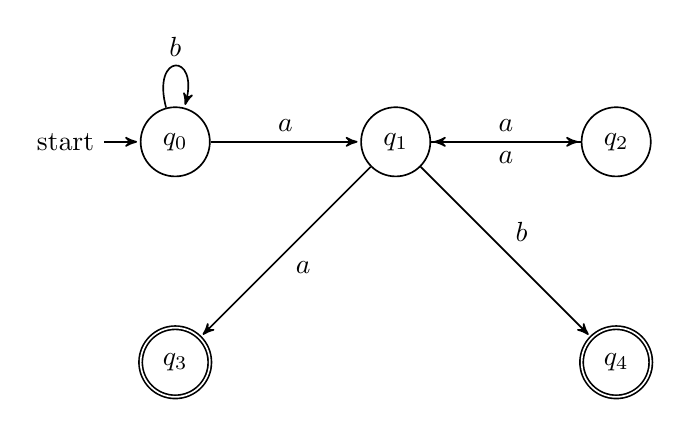
\begin{tikzpicture}[->,>=stealth',shorten >=1pt,auto,node distance=2.8cm,
                    semithick]

  \node[initial,state]   (A)              {$q_0$};
  \node[state]           (B) [right of=A] {$q_1$};
  \node[state]           (C) [right of=B] {$q_2$};
  \node[accepting,state] (D) [below of=A] {$q_3$};
  \node[accepting,state] (E) [below of=C] {$q_4$};

  \path (A) edge [loop above] node {$b$} (A)
            edge              node {$a$} (B)
        (B) edge              node {$a$} (C)
            edge              node {$a$} (D)
            edge              node {$b$} (E)
        (C) edge              node {$a$} (B);
\end{tikzpicture}

\subsection{Problem 2}
\label{sec:orgheadline5}
Given a language \(L=\{w \in \{a,b\}^*\;|\;\#_a(w)=\#_b(w)\}\), show
context-free grammar \(G\) which accepts it.

\subsubsection{Answer 3}
\label{sec:orgheadline4}
\(L\) contains an empty string, thus \(G\) must have the \(S \to \epsilon\) rule.
Also, for any \(a\) is must add a \(b\) somewhere in the word.  There are only
two possible ways to do that: either \(a\) is before \(b\) or the other way
around.  Thus, we need to add two more rules: \(S \to aSbS\) and \(S \to bSaS\).
Using structural induction on the length of the word generated by \(S\) we can
also show that for any word in \(L\) there is a derivation in \(G\).  Hence \(G\)
is given by:

\begin{align*}
  &S \to aSbS \;|\; bSaS \;|\; \epsilon \;.
\end{align*}

\subsection{Problem 3}
\label{sec:orgheadline7}
Show a context-free grammar \(G\) accepting the language \(L\) defined as:
\begin{align*}
  L = \{dw_1dw_2d \dots w_nd &\;|\; n \geq 4 \\
                             &\land \forall k: w_k \in \{a,b,c\}^* \\
                             &\land \exists k: (2 \geq k \geq n-2 \land \#_c(w_{k+2}) = \abs{w_k})\}
\end{align*}

\subsubsection{Answer 4}
\label{sec:orgheadline6}
The words in \(L\) will have to start with at least two repetitions of \(dw\),
followed by the part with a simplified requirement: there will be no
restrictin on the value of \(k\).  Since context-free grammars are closed
under concatenation, I will construct the grammar in steps.

\begin{enumerate}
\item \(G_1\) is the grammar for two repetitions of \(dw\):
\begin{align*}
  &S \to dX \\
  &W \to aW \;|\; bW \;|\; cW \;|\; \epsilon \\
  &X \to WdY \\
  &Y \to WdW \;.
\end{align*}

\item \(G_2\) is the grammar that counts the number of letters in the \(k^{th}\) word
and ensures that \(k+2^{th}\) word has as many \(c\) letters.
\begin{align*}
  &S \to dCT \\
  &W \to aW \;|\; bW \;|\; cW \;|\; \epsilon \\
  &C \to aCc \;|\; bCc \;|\; cCc \;|\; dWd \\
  &T \to TWd \;|\; d \;.
\end{align*}
\end{enumerate}


\(C\) variable is used to count the number of letters in the \(k^{th}\) word.
\(T\) variable is used to add zero or more repetitions of \(dw\) after the
\(k+2^{th}\) word was found.  Followed by the final \(d\).  \(W\) is variable
for generating arbitrary long wrods \(w_i\).


Now, we can combine both grammars:
\begin{align*}
  &S \to dX \\
  &W \to aW \;|\; bW \;|\; cW \;|\; \epsilon \\
  &X \to WdY \\
  &Y \to WdWZ \\
  &Z \to dCT \\
  &C \to aCc \;|\; bCc \;|\; cCc \;|\; dWd \\
  &T \to TWd \;|\; d \;.
\end{align*}

\subsection{Problem 4}
\label{sec:orgheadline10}
Given the grammar \(G\):
\begin{align*}
  &S \to ABC \;|\; bB \;|\; D\\
  &A \to a \;|\; \epsilon \\
  &B \to bB \;|\;\epsilon \\
  &C \to c \\
  &D \to Da \;|\; aDc \;|\; Dc \;|\; ac \;|\; a \;|\; c \;.
\end{align*}


\begin{enumerate}
\item Is \(G\) unambiguous?
\item Give an alternative description to \(L(G)\).
\end{enumerate}

\subsubsection{Answer 5}
\label{sec:orgheadline8}
\(G\) is ambigous, it is possible to derive \(ac\) via:
\begin{enumerate}
\item \(S \to ABC\), \(A \to a\), \(B \to \epsilon\) and \(C \to c\).
\item \(S \to D\), \(D \to ac\).
\end{enumerate}

\subsubsection{Answer 6}
\label{sec:orgheadline9}
\(L(G)\) is actually regular.  If you look at all derivations from \(S\)
separately, then \(ABC\) is equivalent to \((a+\epsilon)b^*c\), \(bB\) is
equivalent to \(b^+\).  And \(D\) is equivalent to \((a+c)^+\).  The later can be
proved by induction on the word length generated by \(D\).

\textbf{Base step:} The word of length 1 can be generated by \(D\), sinc it produces
both \(a\) and \(c\) terminals.

\textbf{Inductive step:} Suppose we can derive the word \((a+c)^+\) of length \(n-1\)
using \(D\) rule, then the word of length \(n\) would be generated by either
the \(D \to Da\) or \(D \to Dc\) rule.

Hence, by induction, \(D\) generates the language \((a+c)^+\).

Now \(L(G)=(a+\epsilon)b^*c+b^++(a+c)^+\), since regular languages are closed
under union.

\subsection{Problem 5}
\label{sec:orgheadline12}
Give a context-free grammar accepting the language
\begin{align*}
  L = \{ x\textbf{+}yz \;| &\; \abs{x} = \abs{y} \\
                         | &\; x, y \in {0, 1}^* \\
                         | &\; \abs{x} \mod 2 = 0 \iff z = \textbf{e} \\
                         | &\; \abs{x} \mod 2 = 1 \iff z = \textbf{o} \}
\end{align*}

\subsubsection{Answer 7}
\label{sec:orgheadline11}
The grammar \(G\) accepting \(L\) can be given as follows:
\begin{align*}
  &S \to Oo \;|\; Ee \\
  &X \to 00 \;|\; 01 \;|\; 10 \;|\; 11 \\
  &E \to XEX \;|\; X+X \\
  &O \to XOX \;|\; 0+0 \;|\; 0+1 \;|\; 1+0 \;|\; 1+1 \;.
\end{align*}


\(O\) variable is responsible for generating odd \(x\) and \(y\) while \(E\) is
responsible for generating even sums.  \(X\) generates all possible pairs of
zeros and ones.  It is easy to get convinced that \(E\) will generate all and
only even sums (since concatenating \(X\) arbitrary number of times will
produce only words of even length).  Similarly, \(E\) will generate all and
only odd sums.

Only odd sums can terminate in \(o\) and only even sums can terminate in \(e\).

\lstset{language=prolog,label= ,caption= ,captionpos=b,numbers=none}
\begin{lstlisting}
even_binary --> "00" ; "11" ; "01" ; "10" ;
               "00" , even_binary ;
               "10" , even_binary ;
               "01" , even_binary ;
               "11" , even_binary.

odd_binary --> "0" ; "1" ; "1", even_binary ; "0", even_binary.

odd_sums --> odd_binary , "+" , odd_binary.

even_sums --> even_binary , "+" , even_binary.

sums --> odd_sums, "o" ; even_sums, "e" .

print_helper(E) :-
    string_codes(X, E),
    (phrase(sums, E) ->
         format('\\item ~w \\textit{accepted}\n', [X])
     ;
     format('\\item ~w \\textit{rejected}\n', [X])).

assignment_15 :-
    format('$$\\begin{itemize}\n', []),
    Candidates = [`101+001o`, `1111+0000e`, `101+001`,
                  `1111+0000`, `abcd`, `1010101`, 
                  `0101+1010o`, `001+110e`],
    maplist(print_helper, Candidates),
    format('\\end{itemize}$$', []).
\end{lstlisting}

\(\begin{itemize}
    \item 101+001o \textit{accepted}
    \item 1111+0000e \textit{accepted}
    \item 101+001 \textit{rejected}
    \item 1111+0000 \textit{rejected}
    \item abcd \textit{rejected}
    \item 1010101 \textit{rejected}
    \item 0101+1010o \textit{rejected}
    \item 001+110e \textit{rejected}
    \end{itemize}\)
\end{document}